\documentclass[11pt]{article}

\usepackage[left=2.5cm, right=2cm, top=0.6cm, bottom=2cm, includehead, includefoot]{geometry}
\usepackage[utf8]{inputenc}
\usepackage[T1]{fontenc}
\usepackage[spanish,es-noindentfirst]{babel}
\usepackage{titlesec}
\usepackage{enumitem}
\usepackage{graphicx}
\usepackage{amsmath}
\usepackage{amsfonts}
\usepackage{amssymb}
\usepackage{parskip}
\usepackage{float}
\usepackage{setspace}
\usepackage{fancyhdr}
\usepackage{needspace}
\usepackage{etoolbox}
\usepackage{booktabs}
\usepackage{array}
\usepackage{xcolor}
\usepackage{tikz}
\usetikzlibrary{shapes.geometric, arrows.meta, positioning, calc, fit, backgrounds, shadows.blur}
\usepackage[hidelinks]{hyperref}

\pagestyle{fancy}
\fancyhf{}
\setlength{\headheight}{63pt}
\setlength{\headsep}{10pt}
\fancyhead[C]{\includegraphics[width=\textwidth]{picture/logo.pdf}}
\renewcommand{\headrulewidth}{0pt}
\fancyfoot[C]{\thepage}
\setlength{\footskip}{18pt}

\setstretch{1.12}
\setlength{\parskip}{0.65em}
\setlist[itemize]{leftmargin=1.35cm, itemsep=0.45em, topsep=0.35em}
\setlist[enumerate]{leftmargin=1.35cm, itemsep=0.45em, topsep=0.35em}

\titleformat{\section}{\normalfont\Large\bfseries}{\thesection}{1em}{}
\titleformat{\subsection}{\normalfont\large\bfseries}{\thesubsection}{1em}{}
\titleformat{\subsubsection}{\normalfont\normalsize\bfseries}{\thesubsubsection}{1em}{}
\preto{\subsection}{\Needspace{10\baselineskip}}
\preto{\subsubsection}{\Needspace{8\baselineskip}}

% Colores y estilos para diagramas TikZ
\definecolor{cazul}{HTML}{1d4ed8}
\definecolor{cverde}{HTML}{059669}
\definecolor{cnaranja}{HTML}{ea580c}
\definecolor{cmorado}{HTML}{7c3aed}
\definecolor{cgris}{HTML}{475569}
\tikzset{
  etapa/.style={rectangle, rounded corners=3pt, draw=#1, fill=#1!8, line width=0.9pt,
                text width=2.7cm, align=center, minimum height=1.05cm, font=\footnotesize},
  flecha/.style={-{Stealth[length=2.4mm]}, line width=0.8pt, draw=cgris},
}

\title{Informe del Proyecto}
\raggedbottom

\begin{document}

\renewcommand{\figurename}{Figura}
\renewcommand{\tablename}{Tabla}
\renewcommand{\thesection}{\Roman{section}}

\begin{center}
    \textbf{\underline{\normalsize PROYECTO FINAL}}
\end{center}

\section{PORTADA}

\begin{center}
    \textbf{UNIVERSIDAD TÉCNICA DE AMBATO}\\
    Facultad de Ingeniería en Sistemas, Electrónica e Industrial\\
    ``Proyecto Académico de Fin de Semestre: Enero -- Julio 2026''
\end{center}

\begin{tabbing}
    \textbf{Unidad de Organización Curricular:}\hspace{0.6cm} \= \kill
    \textbf{Tema:} \> Sistema inteligente de radar vehicular: medición de \\
    \> velocidad multi-vehículo, reconocimiento de placas \\
    \> ecuatorianas y sanción difusa proporcional \\[0.25em]
    \textbf{Carrera:} \> Ingeniería de Software \\[0.25em]
    \textbf{Unidad de Organización Curricular:} \> PROFESIONAL \\[0.25em]
    \textbf{Línea de Investigación:} \> Tecnologías de la Información y Sistemas de Control \\[0.25em]
    \textbf{Nivel y Paralelo:} \> Séptimo ``A'' \\[0.25em]
    \textbf{Alumnos participantes:} \> Paul Velastegui \\
    \> David Manjarres \\[0.25em]
    \textbf{Asignatura:} \> Inteligencia Artificial \\[0.25em]
    \textbf{Docente:} \> Ing. Rubén Nogales, Mg.
\end{tabbing}

\section{INFORME DEL PROYECTO}
\renewcommand{\thesection}{\arabic{section}}
\setcounter{section}{0}

\subsection{Título}
Sistema inteligente de radar vehicular para la medición simultánea de velocidad de
múltiples vehículos, el reconocimiento de placas ecuatorianas y la evaluación difusa
de sanciones proporcionales en un entorno universitario controlado.

\subsection{Resumen}
El proyecto implementa un radar vehicular inteligente orientado al control de
velocidad en una zona universitaria. La solución procesa video en tiempo real o desde
archivo y rastrea \emph{simultáneamente} a todos los vehículos del cuadro mediante un
detector YOLO11 acoplado al algoritmo de seguimiento ByteTrack, lo que permite medir
la velocidad de entre uno y seis vehículos a la vez. La velocidad se estima cuando el
vehículo cruza dos líneas virtuales separadas por una distancia conocida. Para cada
vehículo cercano se detecta la placa con un modelo YOLO, se segmentan sus caracteres
con una red U-Net y se clasifican individualmente con una CNN de 36 clases
alfanuméricas; la lectura se estabiliza por votación temporal entre fotogramas y se
valida con el formato ecuatoriano de tres letras y tres o cuatro dígitos. Los modelos
de reconocimiento, entrenados originalmente en Keras, se convirtieron a formato ONNX
para ejecutarse sobre \texttt{onnxruntime} en Python~3.14 sin TensorFlow. La decisión
disciplinaria se realiza con un sistema difuso de dos etapas: una clasificación
Mamdani (felicitación / normal / multa) y una inferencia Takagi--Sugeno que convierte
el exceso sobre el límite de 20~km/h en horas de indisponibilidad de forma suave,
monótona y proporcional. El sistema registra los eventos, almacena evidencias
visuales, notifica por correo electrónico y expone una interfaz web de monitoreo.

\subsection{Palabras clave}
Visión por computador, seguimiento multi-objeto, reconocimiento de placas, U-Net,
CNN, YOLO, ByteTrack, lógica difusa, Mamdani, Takagi--Sugeno, ONNX, radar vehicular.

\subsection{Objetivos}
\textbf{General:}
\begin{itemize}
    \item Desarrollar un sistema inteligente de radar vehicular que mida la velocidad
    de varios vehículos de forma simultánea, reconozca sus placas ecuatorianas y
    sugiera una sanción proporcional mediante lógica difusa, integrando todo en una
    aplicación web de monitoreo.
\end{itemize}

\textbf{Específicos:}
\begin{itemize}
    \item Implementar el seguimiento multi-vehículo con YOLO11 y ByteTrack para medir
    la velocidad de cada vehículo al cruzar dos líneas virtuales calibradas.
    \item Reconocer la cadena alfanumérica de la placa combinando detección con YOLO,
    segmentación de caracteres con U-Net y clasificación con CNN, validando el formato
    vehicular ecuatoriano.
    \item Desplegar los modelos de reconocimiento mediante ONNX para ejecutarlos sin
    dependencia de TensorFlow, garantizando portabilidad y rendimiento.
    \item Diseñar un sistema de inferencia difusa que clasifique la conducta y calcule
    una sanción estrictamente proporcional al exceso de velocidad.
    \item Presentar los eventos, las evidencias y el razonamiento difuso en una
    interfaz web, con notificación automática por correo de las infracciones.
\end{itemize}

\subsection{Modalidad}
\begin{tabbing}
    \hspace{1cm} \= Presencial.
\end{tabbing}

\subsection{Listado de equipos, materiales y recursos}
\begin{itemize}
    \item Computador con GPU NVIDIA (aceleración CUDA para los detectores YOLO).
    \item Cámara web / teléfono como fuente de video; videos de tránsito del campus.
    \item Entorno de desarrollo Python 3.14.
    \item Internet y material del aula virtual de la asignatura.
    \item Herramientas para generar documentos en formato PDF.
\end{itemize}

\subsubsection*{Dependencias de Python utilizadas}
\begin{itemize}
    \item \textbf{Ultralytics (\texttt{ultralytics}):} detección y seguimiento YOLO11
    de vehículos y placas.
    \item \textbf{ONNX Runtime (\texttt{onnxruntime}):} inferencia de la U-Net de
    segmentación y la CNN de clasificación de caracteres.
    \item \textbf{OpenCV (\texttt{opencv-python}):} captura de video, preprocesamiento,
    enderezado y operaciones geométricas.
    \item \textbf{NumPy (\texttt{numpy}):} representación matricial y operaciones
    vectoriales.
    \item \textbf{scikit-fuzzy (\texttt{scikit-fuzzy}):} funciones de pertenencia del
    sistema difuso.
    \item \textbf{FastAPI / Uvicorn:} backend web y transmisión del video procesado.
    \item \textbf{Matplotlib:} renderizado del razonamiento difuso.
\end{itemize}

\textbf{TAC (Tecnologías para el Aprendizaje y Conocimiento):}

$\square$ Plataformas educativas \quad $\blacksquare$ Aplicaciones educativas \quad
$\blacksquare$ Inteligencia Artificial \quad $\square$ Recursos audiovisuales

\subsection{Planteamiento del problema}
La identificación automática de vehículos por su placa es una aplicación frecuente de
la visión por computador en el control de accesos, la seguridad y el monitoreo de
tránsito \cite{alpr_survey}. En entornos universitarios el control de velocidad es
crítico para la protección peatonal, pero la vigilancia manual es costosa, no genera
evidencia objetiva y no escala cuando circulan varios vehículos a la vez.

El problema abordado es, por tanto, construir un radar que, a partir de una sola
cámara, sea capaz de: (i)~medir la velocidad de \emph{múltiples} vehículos
simultáneamente; (ii)~leer de forma confiable la placa ecuatoriana de cada uno pese a
la distancia, el desenfoque por movimiento y la inclinación; y (iii)~traducir el
exceso de velocidad en una sanción \emph{proporcional} e interpretable, evitando los
saltos bruscos de los umbrales rígidos. Cada uno de estos puntos plantea un reto
técnico distinto: el seguimiento estable de identidades, el reconocimiento robusto de
caracteres y la toma de decisiones bajo variables graduales.

\subsection{Marco de referencia: formato de placas ecuatorianas}
El sistema considera placas ecuatorianas de seis o siete caracteres: tres letras
iniciales seguidas de tres o cuatro dígitos (p.~ej.\ \texttt{ABC-1234}). Esta
estructura se aprovecha como una capa de validación que descarta lecturas anómalas
generadas por ruido visual o regiones que no corresponden a una placa, y permite
aceptar tanto el modelo actual como el antiguo de placa ecuatoriana.

\subsection{Metodología}

\subsubsection{Arquitectura general del sistema}
El sistema se organiza en cuatro bloques: adquisición y seguimiento de video, pipeline
de visión por computador, decisión difusa y backend/frontend de monitoreo. La
Figura~\ref{fig:arquitectura} resume el flujo completo de un evento.

\begin{figure}[H]
    \centering
    \begin{tikzpicture}[node distance=0.55cm and 0.7cm]
        \node[etapa=cazul] (cap) {1. Captura de video (cámara / archivo)};
        \node[etapa=cazul, right=of cap] (track) {2. Seguimiento multi-vehículo \\ YOLO11 + ByteTrack};
        \node[etapa=cazul, right=of track] (vel) {3. Cruce de 2 líneas \\ $\rightarrow$ velocidad};
        \node[etapa=cverde, below=0.9cm of vel] (det) {4. Detección de placa (YOLO)};
        \node[etapa=cverde, left=of det] (ocr) {5. OCR: U-Net + CNN (ONNX)};
        \node[etapa=cverde, left=of ocr] (voto) {6. Votación temporal + formato EC};
        \node[etapa=cmorado, below=0.9cm of voto] (fuzzy) {7. Difuso: Mamdani + Sugeno};
        \node[etapa=cnaranja, right=of fuzzy] (reg) {8. Registro + evidencia};
        \node[etapa=cnaranja, right=of reg] (out) {9. Correo + frontend web};

        \draw[flecha] (cap) -- (track);
        \draw[flecha] (track) -- (vel);
        \draw[flecha] (vel) -- (det);
        \draw[flecha] (det) -- (ocr);
        \draw[flecha] (ocr) -- (voto);
        \draw[flecha] (voto) -- (fuzzy);
        \draw[flecha] (fuzzy) -- (reg);
        \draw[flecha] (reg) -- (out);
    \end{tikzpicture}
    \caption{Flujo general del radar vehicular: del video al evento registrado.}
    \label{fig:arquitectura}
    \vspace{2pt}
    {\footnotesize Fuente: Elaboración propia.}
\end{figure}

\subsubsection{Seguimiento multi-vehículo y medición de velocidad}
A diferencia de un enfoque de un solo vehículo, el sistema rastrea \emph{todos} los
vehículos del cuadro. Cada fotograma se reduce al 50\,\% y se procesa con un detector
YOLO11 en su variante \emph{nano} (clases COCO: automóvil, motocicleta, bus y camión)
\cite{yolo11}, acoplado al algoritmo de seguimiento ByteTrack, que asocia cada
detección con una identidad estable entre fotogramas \cite{bytetrack}. Gracias a estas
identidades, el sistema mantiene un estado independiente por vehículo (cruces, tiempos,
lecturas de placa), lo que habilita la medición simultánea de entre uno y seis
vehículos.

La zona de medición se define con dos líneas virtuales separadas por una distancia
conocida $d$. Para cada vehículo se observa el punto de contacto con el suelo
(centro inferior de su caja). Cuando ese punto cruza la primera línea se registra el
tiempo $t_a$ y cuando cruza la segunda, $t_b$. La velocidad se calcula como:
\begin{equation}
    v = \frac{d}{|t_b - t_a|}\times 3.6 \quad [\text{km/h}],
    \label{eq:velocidad}
\end{equation}
donde el factor $3.6$ convierte de m/s a km/h. Para fuentes de archivo se emplean las
marcas de tiempo del propio video (no el reloj de CPU), de modo que la medición es
exacta aunque el procesamiento sea más lento que el tiempo real.

\paragraph{Criterio de muestreo (Nyquist).} La confiabilidad de la medición depende
del número de fotogramas observados durante el cruce, $N = dt \cdot F_s$, con $F_s$ el
fps efectivo. Con pocos fotogramas el sistema dispone de poca evidencia temporal y la
velocidad puede inflarse; con más fotogramas el error relativo disminuye como
$\approx 1/N$. Esta es la versión temporal del criterio de muestreo: la frecuencia
debe ser suficiente para capturar el fenómeno de interés \cite{szeliski}. De forma
análoga, en el dominio espacial la resolución determina cuántos píxeles cubren la
placa; una placa lejana se reduce a muy pocos píxeles y pierde legibilidad.

\subsubsection{Detección de la placa}
La región de la placa se localiza con un modelo YOLO entrenado para una sola clase
(\emph{License\_Plate}). YOLO se eligió por su detección en una sola etapa, adecuada
para tiempo real \cite{yolo11}. La red redimensiona internamente la entrada a
$416\times416$, pero el recorte de la placa se extrae del fotograma original en su
resolución completa; así las etapas posteriores de segmentación y clasificación
disponen del máximo detalle posible. Cuando la placa recortada es pequeña se amplía
por interpolación cúbica antes del OCR.

\subsubsection{Reconocimiento de la placa: U-Net + CNN}
El reconocimiento se realiza en tres pasos (Figura~\ref{fig:ocr}). Primero, el recorte
de la placa se endereza por rotación estimando la inclinación con la transformada de
Hough (corrección puramente geométrica, sin dependencias adicionales). Segundo, una
red U-Net \cite{unet} de entrada $96\times256\times1$ produce una máscara
probabilística donde cada píxel indica su probabilidad de pertenecer a un carácter; la
máscara se binariza, se extraen contornos y se generan recortes individuales por
carácter. La U-Net \emph{no} clasifica caracteres: su única función es separar a nivel
de píxel las regiones de tinta, lo que generaliza mucho mejor que una umbralización
fija ante placas variadas, sombras o inclinación. Tercero, cada recorte se redimensiona
a $64\times64$ y se clasifica con una CNN de 36 clases (dígitos 0--9 y letras A--Z) de
filosofía VGG con \emph{Global Average Pooling} \cite{cnn_chars}.

\begin{figure}[H]
    \centering
    \begin{tikzpicture}[node distance=0.55cm]
        \node[etapa=cverde] (a) {Recorte de placa (YOLO)};
        \node[etapa=cverde, right=of a] (b) {Enderezado (Hough)};
        \node[etapa=cverde, right=of b] (c) {U-Net $96{\times}256$ \\ máscara de chars};
        \node[etapa=cverde, right=of c] (d) {Cajas + recortes por carácter};
        \node[etapa=cverde, below=0.8cm of d] (e) {CNN $64{\times}64$ \\ 36 clases};
        \node[etapa=cverde, left=of e] (f) {Formato EC \\ 3 letras + 3/4 díg.};
        \node[etapa=cmorado, left=of f] (g) {Texto crudo \\ al votador};
        \draw[flecha] (a)--(b); \draw[flecha] (b)--(c); \draw[flecha] (c)--(d);
        \draw[flecha] (d)--(e); \draw[flecha] (e)--(f); \draw[flecha] (f)--(g);
    \end{tikzpicture}
    \caption{Cadena de reconocimiento de la placa: detección, enderezado, segmentación
    U-Net, clasificación CNN y validación de formato.}
    \label{fig:ocr}
    \vspace{2pt}
    {\footnotesize Fuente: Elaboración propia.}
\end{figure}

\paragraph{Despliegue con ONNX (sin TensorFlow).} Los pesos de la U-Net y de la CNN se
entrenaron originalmente en Keras (formato \texttt{.keras}). Dado que el entorno de
ejecución es Python~3.14 ---donde TensorFlow no dispone de paquetes--- los modelos se
convirtieron una sola vez a formato ONNX y se ejecutan con \texttt{onnxruntime}
\cite{onnxruntime}. Esta decisión elimina la dependencia de TensorFlow, evita el
conflicto de memoria de GPU con PyTorch (usado por YOLO) y mantiene la inferencia del
OCR en CPU, liberando la GPU para el seguimiento.

\subsubsection{Validación de formato y votación temporal}
Como la misma placa se observa en muchos fotogramas mientras el vehículo cruza la zona,
el sistema acumula las lecturas crudas por vehículo y produce un \emph{consenso} por
votación posición a posición ponderada por confianza y por tamaño de la placa (los
fotogramas cercanos pesan más). Sobre ese consenso se aplica la validación de formato
ecuatoriano; sólo se registra un evento cuando el consenso cumple la estructura
\texttt{3~letras + 3/4~dígitos}. La votación corrige los errores de un solo fotograma
(desenfoque, ángulo) y eleva notablemente la precisión final.

\subsubsection{Sistema de inferencia difusa}
La decisión disciplinaria se modela con lógica difusa, adecuada cuando intervienen
variables graduales como la velocidad, en lugar de umbrales rígidos \cite{zadeh}. El
diseño tiene dos etapas (Figura~\ref{fig:fuzzy}):

\begin{enumerate}
    \item \textbf{Clasificación (Mamdani).} Tres conjuntos difusos de velocidad
    ---\emph{felicitación} (0--10), \emph{normal} (10--20) y \emph{multa} ($>$20)---
    determinan la categoría por máxima pertenencia \cite{mamdani}. La pertenencia de
    \emph{multa} es una rampa monótona desde el límite de 20~km/h, lo que evita el
    perfil en ``serrucho'' que produciría el máximo de varios triángulos solapados.
    \item \textbf{Sanción (Takagi--Sugeno).} Sólo cuando la categoría es \emph{multa},
    las horas de indisponibilidad se obtienen con una inferencia Sugeno de orden cero
    \cite{sugeno}: cinco sub-niveles de severidad (leve\dots extrema) que teselan el
    rango 20--40~km/h, cada uno con un consecuente \emph{singleton} creciente. La
    salida es el promedio ponderado
    \begin{equation}
        H(v) = \frac{\sum_i \mu_i(v)\, c_i}{\sum_i \mu_i(v)},
        \label{eq:sugeno}
    \end{equation}
    donde $\mu_i(v)$ es la pertenencia al sub-nivel $i$ y $c_i$ su singleton en horas.
\end{enumerate}

El motivo de usar Sugeno para la sanción es técnico: el centroide de Mamdani introduce
mesetas y micro-descensos no monótonos cerca de los bordes de cada conjunto, mientras
que el promedio ponderado de singletons~\eqref{eq:sugeno} produce una salida
\emph{estrictamente monótona y suave}, que es precisamente la proporcionalidad
requerida ---a mayor exceso sobre 20~km/h, mayor sanción---. Las funciones de
pertenencia empleadas son triangulares $\mu_{tri}(x;a,b,c)$ y trapezoidales
$\mu_{trap}(x;a,b,c,d)$ estándar.

\begin{figure}[H]
    \centering
    \begin{tikzpicture}[node distance=0.6cm and 0.9cm]
        \node[etapa=cmorado] (v) {Velocidad $v$};
        \node[etapa=cmorado, right=1.4cm of v] (cls) {Mamdani: \\ felicitación / normal / multa};
        \node[etapa=cgris, above right=0.1cm and 1.1cm of cls] (nomulta) {$\neq$ multa \\ $\rightarrow 0$ h};
        \node[etapa=cmorado, below right=0.1cm and 1.1cm of cls] (sug) {Sugeno: $H(v)=\frac{\sum \mu_i c_i}{\sum \mu_i}$};
        \node[etapa=cnaranja, right=1.1cm of sug] (h) {Horas de \\ indisponibilidad};
        \draw[flecha] (v)--(cls);
        \draw[flecha] (cls)-- (nomulta);
        \draw[flecha] (cls)-- (sug);
        \draw[flecha] (sug)--(h);
    \end{tikzpicture}
    \caption{Decisión difusa en dos etapas: clasificación Mamdani y sanción
    proporcional Takagi--Sugeno.}
    \label{fig:fuzzy}
    \vspace{2pt}
    {\footnotesize Fuente: Elaboración propia.}
\end{figure}

\subsubsection{Backend, frontend y notificación}
El backend, construido con FastAPI, integra el pipeline de visión, transmite el video
procesado y emite eventos. Por cada evento guarda el fotograma con la placa y la
velocidad, registra el evento y dispara una notificación por correo con la evidencia y
el razonamiento difuso. El frontend permite seleccionar la fuente, arrastrar las líneas
de medición, observar el video en vivo, revisar el historial de eventos con miniaturas
y visualizar el detalle de cada evento.

\subsection{Conjuntos de datos y entrenamiento}
La trazabilidad del origen de los datos es parte central del informe. Los tres modelos
de reconocimiento se entrenaron con conjuntos públicos alojados en Roboflow Universe,
todos bajo licencia CC~BY~4.0.

\subsubsection{Detección de placa}
El detector de placa se entrenó con el conjunto público \emph{License Plate
Recognition} (v13) de Roboflow Universe, de origen internacional y una sola clase
\emph{License\_Plate}, con 101\,866 imágenes generadas por aumento de datos a partir de
$\sim$7\,276 imágenes fuente \cite{ds_placas}. El reparto se muestra en la
Tabla~\ref{tab:ds_placas}. Sobre estos datos se entrenó una red YOLO en variante
\emph{nano}, con entrada $416\times416$. El uso de un conjunto amplio busca que el
detector aprenda la apariencia general de una placa; la validación de formato adapta la
lectura final al contexto ecuatoriano.

\begin{table}[H]
    \centering
    \caption{Conjunto de detección de placas (Roboflow, v13) \cite{ds_placas}.}
    \label{tab:ds_placas}
    \begin{tabular}{lr}
        \toprule
        \textbf{Partición} & \textbf{Número de imágenes} \\
        \midrule
        Entrenamiento & 98\,798 \\
        Validación    & 2\,048 \\
        Prueba        & 1\,020 \\
        \midrule
        Total         & 101\,866 \\
        \bottomrule
    \end{tabular}
\end{table}

\subsubsection{Clasificación de caracteres (CNN)}
El clasificador CNN se entrenó con recortes alfanuméricos provenientes de un conjunto
de placas del Reino Unido \cite{ds_uk} y un conjunto de placas de Brasil
\cite{ds_brasil}, sobre una entrada de $64\times64$ en escala de grises y 36 clases.
El entrenamiento empleó aumento de datos, pesos por clase y pérdida focal
\cite{focal_loss} para compensar el desbalance natural entre caracteres frecuentes y
poco frecuentes. Pruebas exploratorias confirmaron que $64\times64$ preserva mejor los
rasgos discriminantes que $32\times32$ o $48\times48$ (Tabla~\ref{tab:resolucion}).

\subsubsection{Segmentación de caracteres (U-Net)}
Para la U-Net se combinaron un conjunto base de la India, recortes reales de placas
ecuatorianas obtenidos del dataset de detección ecuatoriano \cite{ds_ec}, y
subconjuntos de Brasil \cite{ds_brasil} y Reino Unido \cite{ds_uk}, además de un
conjunto específico de segmentación de caracteres \cite{ds_seg}. La función de pérdida
combinó entropía cruzada binaria ponderada y pérdida Dice, con un mapa de pesos que
penaliza los separadores entre caracteres vecinos para evitar que dos caracteres se
fusionen en un mismo recorte.

\subsection{Resultados y discusión}

\subsubsection{Detección de placa}
El detector YOLO alcanzó los valores de la Tabla~\ref{tab:det}. Una precisión de
$0.990$ y un mAP@50 de $0.950$ indican que la región de la placa se localiza de forma
confiable, condición necesaria para que la segmentación y la clasificación operen sobre
un recorte adecuado. El mAP@50--95 de $0.661$, más bajo por su exigencia de ajuste fino
de la caja, es suficiente para el recorte de placa, ya que la segmentación posterior no
requiere un ajuste perfecto de bordes.

\begin{table}[H]
    \centering
    \caption{Métricas del detector YOLO de placas.}
    \label{tab:det}
    \begin{tabular}{lr}
        \toprule
        \textbf{Métrica} & \textbf{Valor} \\
        \midrule
        Precisión        & 0.990 \\
        Exhaustividad (\emph{recall}) & 0.924 \\
        mAP@50           & 0.950 \\
        mAP@50--95       & 0.661 \\
        \bottomrule
    \end{tabular}
\end{table}

\subsubsection{Clasificación de caracteres}
El clasificador CNN obtuvo una exactitud global de $0.9132$ sobre un conjunto de prueba
independiente, con métricas macro y ponderadas superiores a $0.90$
(Tabla~\ref{tab:cnn}). Las clases con menor desempeño corresponden a caracteres
visualmente ambiguos (p.~ej.\ O/0, I/1), coherente con la dificultad del problema. La
comparación de resoluciones de entrada (Tabla~\ref{tab:resolucion}) justifica la
elección de $64\times64$.

\begin{table}[H]
    \centering
    \caption{Métricas globales del clasificador CNN de caracteres.}
    \label{tab:cnn}
    \begin{tabular}{lccc}
        \toprule
        \textbf{Métrica} & \textbf{Precisión} & \textbf{Recall} & \textbf{F1} \\
        \midrule
        Promedio macro     & 0.9140 & 0.9040 & 0.9075 \\
        Promedio ponderado & 0.9143 & 0.9132 & 0.9129 \\
        Exactitud global   & \multicolumn{3}{c}{0.9132} \\
        \bottomrule
    \end{tabular}
\end{table}

\begin{table}[H]
    \centering
    \caption{Comparación de resolución de entrada para la clasificación.}
    \label{tab:resolucion}
    \begin{tabular}{lcl}
        \toprule
        \textbf{Resolución} & \textbf{Exactitud} & \textbf{Observación} \\
        \midrule
        $32\times32$ & 0.81   & Mayor pérdida de detalle en trazos finos \\
        $48\times48$ & 0.87   & Mejora parcial, aún con confusiones visuales \\
        $64\times64$ & 0.9132 & Mejor preservación de rasgos discriminantes \\
        \bottomrule
    \end{tabular}
\end{table}

\subsubsection{Segmentación}
La U-Net se evaluó con el coeficiente Dice e IoU binario, métricas apropiadas para
segmentación de máscaras, alcanzando un Dice cercano a $0.91$. A diferencia de la
clasificación, aquí no corresponde una matriz de confusión multiclase porque la salida
es una máscara binaria de carácter/fondo. La segmentación aprendida aporta robustez
frente a inclinación e iluminación, lo que se traduce en una mejor generalización a
placas no vistas durante el entrenamiento.

\subsubsection{Funcionamiento del radar en eventos reales}
La aplicación integra las etapas de video, medición de velocidad, lectura de placa,
cálculo de sanción y visualización. La Figura~\ref{fig:tiempo_real} muestra el
dashboard de monitoreo en tiempo real, con las dos líneas de medición, el panel de
configuración de la fuente, la última placa leída con su velocidad y el historial de
eventos con miniaturas.

\begin{figure}[H]
    \centering
    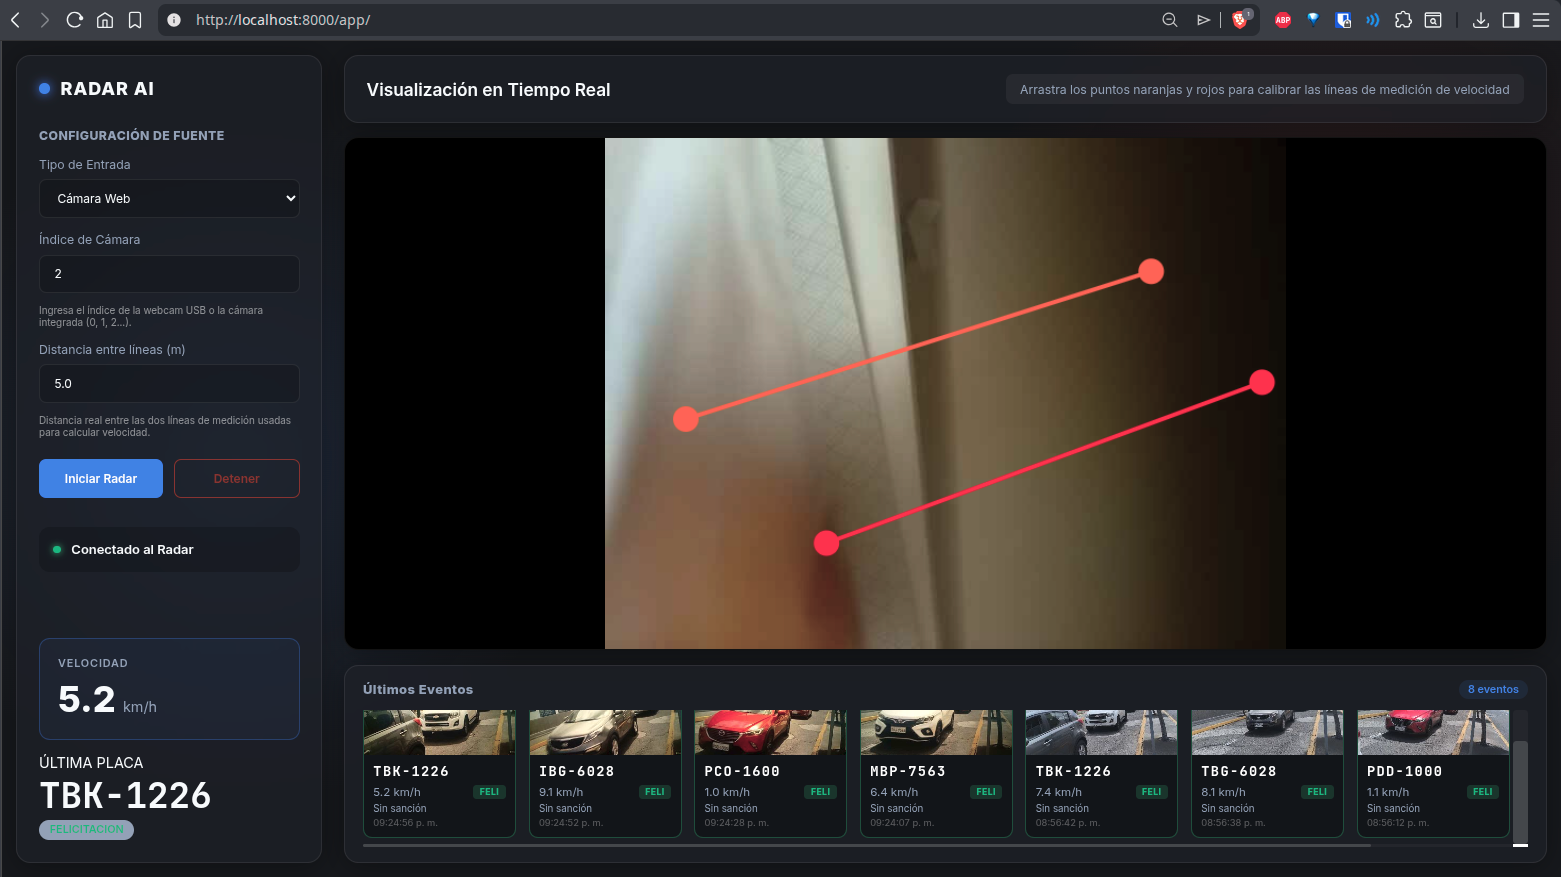
\includegraphics[width=0.92\textwidth]{img/prueba-sistema-tiempo-real.png}
    \caption{Dashboard de monitoreo en tiempo real con las líneas de medición, el panel
    de fuente y el historial de eventos.}
    \label{fig:tiempo_real}
    \vspace{2pt}
    {\footnotesize Fuente: Elaboración propia.}
\end{figure}

En una evaluación sobre un video de tránsito del campus, el radar midió la velocidad de
cuatro vehículos y registró los cuatro con su placa leída, de forma repetible entre
ejecuciones, demostrando la operación multi-vehículo. La Figura~\ref{fig:evento}
presenta el detalle de un evento: el fotograma capturado, la placa, la velocidad, la
clasificación difusa y el razonamiento asociado.

\begin{figure}[H]
    \centering
    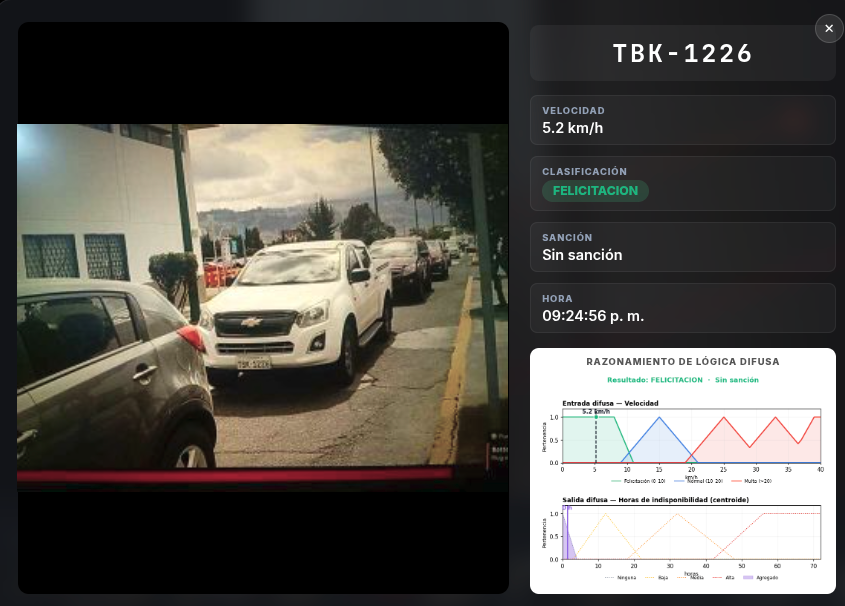
\includegraphics[width=0.80\textwidth]{img/particular-event-data.png}
    \caption{Detalle de un evento: placa \texttt{TBK-1226}, velocidad 5.2~km/h,
    clasificación \emph{felicitación} (sin sanción) y razonamiento difuso.}
    \label{fig:evento}
    \vspace{2pt}
    {\footnotesize Fuente: Elaboración propia.}
\end{figure}

\subsubsection{Sanción difusa proporcional}
La Figura~\ref{fig:difuso} muestra el razonamiento difuso para un caso de multa: el
panel superior contiene las pertenencias de velocidad con la categoría \emph{multa}
como rampa limpia, y el panel inferior la curva de sanción $H(v)$, que es nula en la
zona permitida ($\le$20~km/h) y crece de forma suave y monótona. La
Tabla~\ref{tab:sancion} confirma la proporcionalidad: la sanción aumenta
estrictamente con la velocidad, desde cero en el límite hasta cerca del máximo de tres
días a 40~km/h.

\begin{figure}[H]
    \centering
    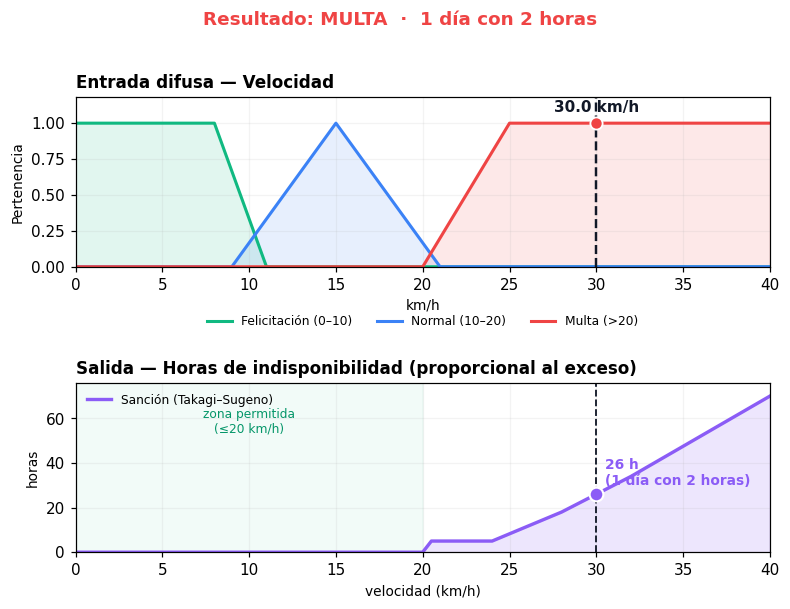
\includegraphics[width=0.82\textwidth]{img/difuso_sancion.png}
    \caption{Razonamiento difuso para un evento de multa a 30~km/h: pertenencias de
    velocidad (arriba) y curva de sanción proporcional $H(v)$ (abajo).}
    \label{fig:difuso}
    \vspace{2pt}
    {\footnotesize Fuente: Elaboración propia.}
\end{figure}

\begin{table}[H]
    \centering
    \caption{Sanción sugerida según la velocidad (salida Takagi--Sugeno).}
    \label{tab:sancion}
    \begin{tabular}{lcl}
        \toprule
        \textbf{Velocidad} & \textbf{Horas} & \textbf{Equivalente} \\
        \midrule
        $\le 20$ km/h & 0  & Sin sanción (zona permitida) \\
        21 km/h & 5  & 5 horas \\
        25 km/h & 8  & 8 horas \\
        30 km/h & 26 & $\approx$ 1 día \\
        35 km/h & 48 & 2 días \\
        40 km/h & 70 & $\approx$ 3 días \\
        \bottomrule
    \end{tabular}
\end{table}

\subsubsection{Notificación por correo}
Cada infracción genera un correo automático con la evidencia del evento, la placa, la
velocidad, la clasificación y el razonamiento difuso, como muestran las
Figuras~\ref{fig:email1} y~\ref{fig:email2}. Esto convierte la detección en un
registro accionable y trazable.

\begin{figure}[H]
    \centering
    \begin{minipage}[t]{0.48\textwidth}
        \centering
        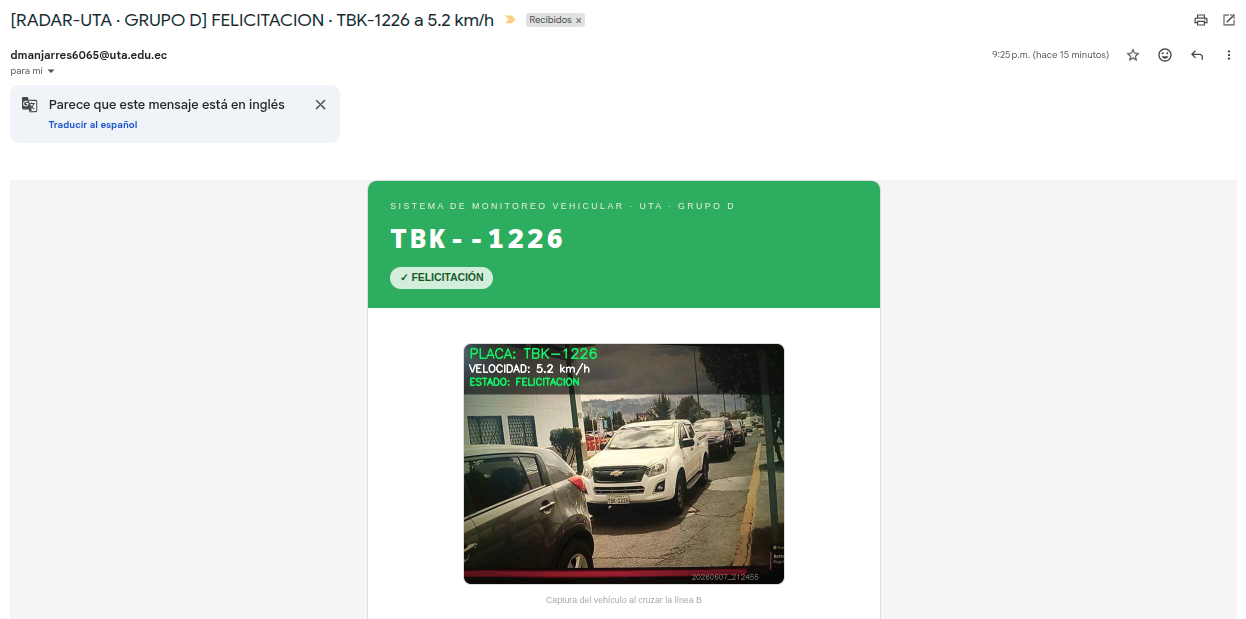
\includegraphics[width=\textwidth]{img/email-1.png}
        \\[3pt]\small (a)
    \end{minipage}
    \hfill
    \begin{minipage}[t]{0.48\textwidth}
        \centering
        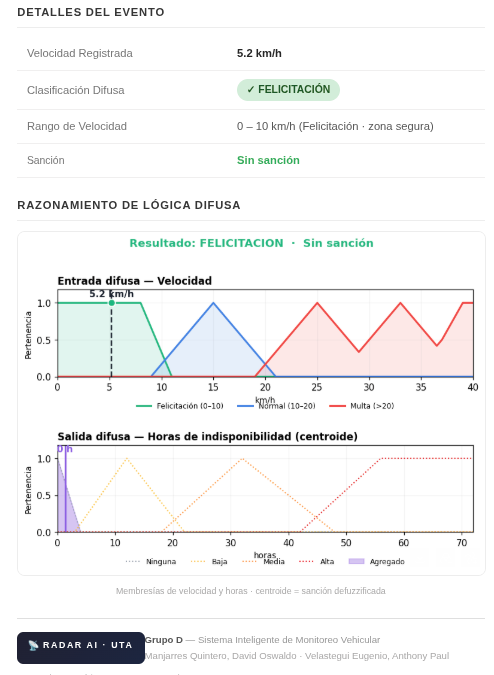
\includegraphics[width=\textwidth]{img/email-2.png}
        \\[3pt]\small (b)
    \end{minipage}
    \caption{Correos de notificación generados automáticamente ante una infracción, con
    evidencia visual y datos del evento.}
    \label{fig:email1}\label{fig:email2}
    \vspace{2pt}
    {\footnotesize Fuente: Elaboración propia.}
\end{figure}

\subsubsection{Discusión}
Los resultados muestran que la solución integra adecuadamente la visión por computador
y la decisión difusa. El seguimiento con ByteTrack permite el caso multi-vehículo sin
confundir identidades, y la votación temporal eleva la confiabilidad de la lectura por
encima de la de un solo fotograma. La segmentación con U-Net aporta robustez frente a
placas variadas, aunque su desempeño final sigue condicionado por la calidad del
recorte, la iluminación y la inclinación. En el módulo difuso, el uso de Takagi--Sugeno
para la sanción garantiza una salida monótona y proporcional, superando las mesetas y
micro-descensos del centroide de Mamdani. Finalmente, el despliegue con ONNX demuestra
que es posible reutilizar modelos entrenados en Keras dentro de un entorno moderno sin
TensorFlow, manteniendo el rendimiento y separando el uso de GPU (seguimiento) del de
CPU (reconocimiento).

\subsection{Habilidades blandas empleadas}
$\blacksquare$ Trabajo en equipo \quad $\blacksquare$ Responsabilidad \quad
$\blacksquare$ Pensamiento crítico \quad $\blacksquare$ Resolución de problemas

\subsection{Conclusiones}
\begin{itemize}
    \item Se desarrolló un radar vehicular funcional que mide la velocidad de varios
    vehículos de forma simultánea mediante YOLO11 y ByteTrack, y registra cada uno con
    su placa y su sanción.
    \item El reconocimiento de placas en cascada (detección YOLO, segmentación U-Net y
    clasificación CNN) con validación de formato ecuatoriano y votación temporal logra
    lecturas confiables sobre placas variadas, no solo las vistas en entrenamiento.
    \item La conversión de los modelos a ONNX permitió ejecutar el OCR en Python~3.14
    sin TensorFlow, eliminando conflictos de dependencias y de memoria de GPU.
    \item El sistema difuso de dos etapas (clasificación Mamdani + sanción Sugeno)
    produce una sanción estrictamente monótona y proporcional al exceso sobre 20~km/h,
    corrigiendo el comportamiento no monótono de un esquema basado únicamente en el
    centroide de Mamdani.
    \item La arquitectura modular y la interfaz web con evidencia por etapa facilitan
    auditar el origen de cualquier error: detección, segmentación, clasificación,
    validación o decisión difusa.
\end{itemize}

\subsection{Recomendaciones}
\begin{itemize}
    \item Calibrar la distancia entre líneas y su posición según la geometría real de
    la cámara; un fps efectivo bajo o una distancia mal medida degradan la exactitud de
    la velocidad.
    \item Para máxima legibilidad de placas, ubicar la zona de medición donde el
    vehículo se observe grande y de frente; las placas lejanas pierden píxeles y
    legibilidad por el límite de muestreo espacial.
    \item Como trabajo futuro, reentrenar el clasificador con más recortes reales de
    placas ecuatorianas para reducir las confusiones entre caracteres similares, y
    explorar un detector de caracteres de extremo a extremo que evite la etapa de
    segmentación.
\end{itemize}

\subsection{Referencias bibliográficas}
{
    \renewcommand{\refname}{}
    \vspace{-1.5em}
    \begin{thebibliography}{99}

    \bibitem{alpr_survey}
    J. Shashirangana, H. Padmasiri, D. Meedeniya, and C. Perera, ``Automated license
    plate recognition: A survey on methods and techniques,'' \emph{IEEE Access},
    vol.~9, pp.~11\,203--11\,225, 2021.

    \bibitem{yolo11}
    G. Jocher and J. Qiu, ``Ultralytics YOLO11,'' Ultralytics, 2024. [En línea].
    Disponible: \url{https://docs.ultralytics.com/models/yolo11/}

    \bibitem{bytetrack}
    Y. Zhang \emph{et al.}, ``ByteTrack: Multi-object tracking by associating every
    detection box,'' in \emph{Proc. European Conf. Computer Vision (ECCV)}, 2022,
    pp.~1--21.

    \bibitem{szeliski}
    R. Szeliski, \emph{Computer Vision: Algorithms and Applications}, 2nd~ed. Cham,
    Switzerland: Springer, 2022.

    \bibitem{ds_placas}
    Roboflow Universe Projects, ``License Plate Recognition Dataset (v13),'' Roboflow
    Universe, CC~BY~4.0, 2026. [En línea]. Disponible:
    \url{https://universe.roboflow.com/roboflow-universe-projects/license-plate-recognition-rxg4e/dataset/13}

    \bibitem{unet}
    O. Ronneberger, P. Fischer, and T. Brox, ``U-Net: Convolutional networks for
    biomedical image segmentation,'' in \emph{Medical Image Computing and
    Computer-Assisted Intervention (MICCAI)}, 2015, pp.~234--241.

    \bibitem{cnn_chars}
    M. Salemdeeb and S. Ertürk, ``Full depth CNN classifier for handwritten and license
    plate characters recognition,'' \emph{PeerJ Computer Science}, vol.~7, Art.~e576,
    2021.

    \bibitem{focal_loss}
    T.-Y. Lin, P. Goyal, R. Girshick, K. He, and P. Dollár, ``Focal loss for dense
    object detection,'' in \emph{Proc. IEEE Int. Conf. Computer Vision (ICCV)}, 2017,
    pp.~2980--2988.

    \bibitem{ds_uk}
    University-UK, ``EN Dataset (v4),'' Roboflow Universe, CC~BY~4.0, 2026. [En línea].
    Disponible: \url{https://universe.roboflow.com/university-uk/en-t0yqi/dataset/4}

    \bibitem{ds_brasil}
    Guilhermecoleta, ``Plate OCR Dataset (v4),'' Roboflow Universe, CC~BY~4.0, 2026.
    [En línea]. Disponible:
    \url{https://universe.roboflow.com/guilhermecoleta/plate-ocr-wb6jn/dataset/4}

    \bibitem{ds_seg}
    Student-Tfefc, ``LPR Character Segmentation Dataset (v3),'' Roboflow Universe,
    CC~BY~4.0, 2026. [En línea]. Disponible:
    \url{https://universe.roboflow.com/student-tfefc/lpr-character-segmentation/dataset/3}

    \bibitem{ds_ec}
    Wilsons-Workspace-Andqz, ``Modelo DeteccionPlacasEc Dataset (v3),'' Roboflow
    Universe, CC~BY~4.0, 2026. [En línea]. Disponible:
    \url{https://universe.roboflow.com/wilsons-workspace-andqz/modelo_deteccionplacasec/dataset/3}

    \bibitem{onnxruntime}
    ONNX Runtime developers, ``ONNX Runtime,'' Microsoft, 2024. [En línea]. Disponible:
    \url{https://onnxruntime.ai/}

    \bibitem{zadeh}
    L. A. Zadeh, ``Fuzzy sets,'' \emph{Information and Control}, vol.~8, no.~3,
    pp.~338--353, 1965.

    \bibitem{mamdani}
    E. H. Mamdani and S. Assilian, ``An experiment in linguistic synthesis with a fuzzy
    logic controller,'' \emph{Int. J. Man-Machine Studies}, vol.~7, no.~1, pp.~1--13,
    1975.

    \bibitem{sugeno}
    T. Takagi and M. Sugeno, ``Fuzzy identification of systems and its applications to
    modeling and control,'' \emph{IEEE Trans. Systems, Man, and Cybernetics},
    vol.~SMC-15, no.~1, pp.~116--132, 1985.

    \bibitem{reglamento}
    Presidencia de la República del Ecuador, ``Reglamento a la Ley de Transporte
    Terrestre, Tránsito y Seguridad Vial,'' Registro Oficial Suplemento~731, Ecuador,
    2012, última reforma 2017.

    \bibitem{traffic_safety}
    J. Wang, C. Zhao, and Z. Liu, ``Can historical accident data improve sustainable
    urban traffic safety? A predictive modeling study,'' \emph{Sustainability}, vol.~16,
    Art.~no.~9642, 2024.

    \end{thebibliography}
}

\end{document}
